\documentclass[12pt,t]{beamer}
\usepackage{graphicx}
\setbeameroption{hide notes}
\setbeamertemplate{note page}[plain]
\usepackage{listings}

% header.tex: boring LaTeX/Beamer details + macros

% get rid of junk
\usetheme{default}
\beamertemplatenavigationsymbolsempty
\hypersetup{pdfpagemode=UseNone} % don't show bookmarks on initial view


% font
\usepackage{fontspec}
\setsansfont
  [ ExternalLocation = fonts/ ,
    UprightFont = *-regular ,
    BoldFont = *-bold ,
    ItalicFont = *-italic ,
    BoldItalicFont = *-bolditalic ]{texgyreheros}
\setbeamerfont{note page}{family*=pplx,size=\footnotesize} % Palatino for notes
% "TeX Gyre Heros can be used as a replacement for Helvetica"
% I've placed them in fonts/; alternatively you can install them
% permanently on your system as follows:
%     Download http://www.gust.org.pl/projects/e-foundry/tex-gyre/heros/qhv2.004otf.zip
%     In Unix, unzip it into ~/.fonts
%     In Mac, unzip it, double-click the .otf files, and install using "FontBook"

% named colors
\definecolor{offwhite}{RGB}{255,250,240}
\definecolor{gray}{RGB}{155,155,155}

\ifx\notescolors\undefined % slides
  \definecolor{foreground}{RGB}{255,255,255}
  \definecolor{background}{RGB}{24,24,24}
  \definecolor{title}{RGB}{107,174,214}
  \definecolor{subtitle}{RGB}{128,128,214}
  \definecolor{hilit}{RGB}{102,255,204}
  \definecolor{vhilit}{RGB}{255,111,207}
  \definecolor{lolit}{RGB}{155,155,155}
  \definecolor{myyellow}{rgb}{1,1,0.7}
\else % notes
  \definecolor{background}{RGB}{255,255,255}
  \definecolor{foreground}{RGB}{24,24,24}
  \definecolor{title}{RGB}{27,94,134}
  \definecolor{subtitle}{RGB}{22,175,124}
  \definecolor{hilit}{RGB}{122,0,128}
  \definecolor{vhilit}{RGB}{255,0,128}
  \definecolor{lolit}{RGB}{95,95,95}
\fi
\definecolor{nhilit}{RGB}{128,0,128}  % hilit color in notes
\definecolor{nvhilit}{RGB}{255,0,128} % vhilit for notes

\newcommand{\hilit}{\color{hilit}}
\newcommand{\vhilit}{\color{vhilit}}
\newcommand{\nhilit}{\color{nhilit}}
\newcommand{\nvhilit}{\color{nvhilit}}
\newcommand{\lolit}{\color{lolit}}

% use those colors
\setbeamercolor{titlelike}{fg=title}
\setbeamercolor{subtitle}{fg=subtitle}
\setbeamercolor{institute}{fg=lolit}
\setbeamercolor{normal text}{fg=foreground,bg=background}
\setbeamercolor{item}{fg=foreground} % color of bullets
\setbeamercolor{subitem}{fg=lolit}
\setbeamercolor{itemize/enumerate subbody}{fg=lolit}
\setbeamertemplate{itemize subitem}{{\textendash}}
\setbeamerfont{itemize/enumerate subbody}{size=\footnotesize}
\setbeamerfont{itemize/enumerate subitem}{size=\footnotesize}

% page number
\setbeamertemplate{footline}{%
    \raisebox{5pt}{\makebox[\paperwidth]{\hfill\makebox[20pt]{\lolit
          \scriptsize\insertframenumber}}}\hspace*{5pt}}

% add a bit of space at the top of the notes page
\addtobeamertemplate{note page}{\setlength{\parskip}{12pt}}

% default link color
\hypersetup{colorlinks, urlcolor={hilit}}

\ifx\notescolors\undefined % slides
  % set up listing environment
  \lstset{language=bash,
          basicstyle=\ttfamily\scriptsize,
          frame=single,
          commentstyle=,
          backgroundcolor=\color{darkgray},
          showspaces=false,
          showstringspaces=false
          }
\else % notes
  \lstset{language=bash,
          basicstyle=\ttfamily\scriptsize,
          frame=single,
          commentstyle=,
          backgroundcolor=\color{offwhite},
          showspaces=false,
          showstringspaces=false
          }
\fi

% a few macros
\newcommand{\bi}{\begin{itemize}}
\newcommand{\bbi}{\vspace{24pt} \begin{itemize} \itemsep8pt}
\newcommand{\ei}{\end{itemize}}
\newcommand{\ig}{\includegraphics}
\newcommand{\subt}[1]{{\footnotesize \color{subtitle} {#1}}}
\newcommand{\ttsm}{\tt \small}
\newcommand{\ttfn}{\tt \footnotesize}
\newcommand{\figh}[2]{\centerline{\includegraphics[height=#2\textheight]{#1}}}
\newcommand{\figw}[2]{\centerline{\includegraphics[width=#2\textwidth]{#1}}}


%%%%%%%%%%%%%%%%%%%%%%%%%%%%%%%%%%%%%%%%%%%%%%%%%%%%%%%%%%%%%%%%%%%%%%
% end of header
%%%%%%%%%%%%%%%%%%%%%%%%%%%%%%%%%%%%%%%%%%%%%%%%%%%%%%%%%%%%%%%%%%%%%%

% title info
\title{Genetic analysis of \\ high-throughput phenotypes}
\subtitle{Challenges and opportunities}
\author{\href{http://kbroman.org}{Karl Broman}}
\institute{Biostatistics \& Medical Informatics, UW{\textendash}Madison}
\date{\href{http://kbroman.org}{\tt \scriptsize \color{foreground} kbroman.org}
\\[-4pt]
\href{https://github.com/kbroman}{\tt \scriptsize \color{foreground} github.com/kbroman}
\\[-4pt]
\href{https://twitter.com/kwbroman}{\tt \scriptsize \color{foreground} @kwbroman}
\\[2pt]
\scriptsize {\lolit Slides:} \href{http://bit.ly/sgn2017}{\tt \scriptsize
  \color{foreground} bit.ly/sgn2017}
}


\begin{document}

% title slide
{
\setbeamertemplate{footline}{} % no page number here
\frame{
  \titlepage

  \hfill 
\includegraphics[height=6mm]{Figs/cc-zero.png}

  \note{These are slides for a talk that I gave at the Workshop on
    Systems Genetics for Neurodegenerative Disease in Frauenchiemsee,
    Germany, on 27 Aug 2017

    Source: {\tt https://github.com/kbroman/Talk\_SGN2017} \\
    Slides: {\tt http://bit.ly/sgn2017}
    }

}
}


\begin{frame}[c]{}

\vspace*{-1mm} \hspace*{-2mm}
\figw{Figs/inbredmice.jpg}{1.2}

\end{frame}


\begin{frame}{}

\vspace*{18mm}

\centerline{
\begin{minipage}[t]{50mm}
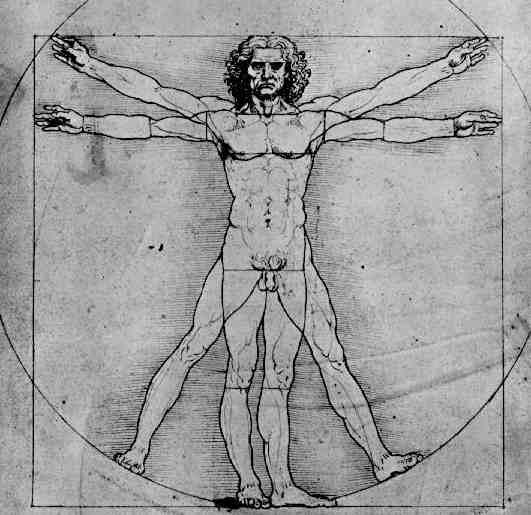
\includegraphics[height=50mm]{Figs/da-vinci-man.jpg}
\end{minipage}
\hspace{15mm}
\begin{minipage}[t]{50mm}
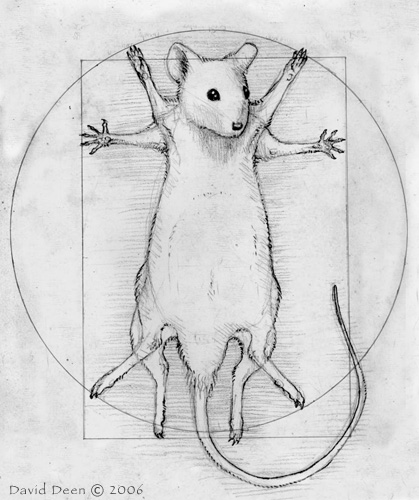
\includegraphics[height=50mm]{Figs/vitruvian_mouse.jpg}
\hspace{5mm}
\href{http://daviddeen.com}{\scriptsize \lolit \tt daviddeen.com}
\end{minipage}
}
\end{frame}


\begin{frame}[c]{Intercross}
\figh{Figs/intercross.pdf}{1.0}
\end{frame}


\begin{frame}[c]{Data}

\hspace{0mm}

\figw{Figs/data_fig.png}{1.15}
\end{frame}



\begin{frame}[c]{QTL mapping}

\vspace{5mm}
\figh{Figs/lodcurve_insulin_with_effects.pdf}{0.9}
\end{frame}


\begin{frame}[c]{\href{https://www.biostat.wisc.edu/~kbroman/presentations/SGN2017/lod_and_effect}{\color{title} Genome scan}}

\figh{Figs/lod_interactive.png}{0.85}

\note{
  Here is a plot of the scan across the genome.

  Think of the test statistic, ``LOD score'', as sort of like the
  --log$_{10}$ p-value, though really it's a log$_{10}$ likelihood
  ratio.

  This links to an interactive plot, where you can explore the
  genotype-phenotype associations across the genome.
}
\end{frame}




\begin{frame}[c]{Permutation test}

\figw{Figs/permtest_illustration.pdf}{0.9}

\note{
  A key issue in this business is the need to adjust for the multiple
  statistical tests performed: that we did a ``scan'' across the
  genome, testing for the genotype/phenotype association at each
  marker.

  To deal with this, we derive the distribution of the genome-wide
  maximum test statistic under the ``global'' null hypothesis that the
  phenotype is totally unrelated to the genotypes.

  To determine that null distribution, we shuffle the phenotype
  relative to the genotypes, calculate the test statistics across the
  genome, derive the maximum test statistic, and repeat many times.
}
\end{frame}






\begin{frame}[c]{\href{https://www.biostat.wisc.edu/~kbroman/presentations/SGN2017/perm_test}{\color{title} Permutation test}}

\figw{Figs/perm_test.png}{0.9}

\note{
  This is an interactive illustration of a permutation test.

  Click the ``Randomize'' button to shuffle the phenotypes and re-draw
  the LOD curves; click the ``back'' button to go back.
}
\end{frame}




\begin{frame}[c]{Histogram of permutation results}

\figw{Figs/permtest_hist.pdf}{0.9}

\note{
  Here's a histogram of the results of a permutation test with 10,000 replicates.

  A 5\% significance threshold can be taken to be the 95th percentile
  of the results, which is about 3.9 in this case.
}
\end{frame}


\begin{frame}[c]{Modeling multiple QTL}

\vspace{-20mm}

  \bbi
\item Reduce residual variation $\longrightarrow$ increased power
\item Separate linked QTL
\item Identify interactions among QTL {\lolit (epistasis)}
  \ei
\end{frame}





\begin{frame}[c]{Epistasis in F$_\text{2}$}

\figw{Figs/epistasis_f2.pdf}{1.0}

\end{frame}




\begin{frame}[c]{Congenic line}

\figw{Figs/congenic.pdf}{1.0}

\end{frame}



\begin{frame}[c]{Improving precision}

  \vspace{-20mm}

  \bbi
\item more recombinations
\item more individuals
\item more precise phenotype
\item lower-level phenotypes
\bi
\item transcripts, proteins, metabolites
  \ei
  \ei

\end{frame}



\begin{frame}[c]{Advanced intercross lines}

  \figh{Figs/ail.pdf}{0.9}

\end{frame}


\begin{frame}[c]{Recombinant inbred lines}

  \figh{Figs/rilines.pdf}{0.9}

\end{frame}


\begin{frame}[c]{Collaborative Cross}

  \figh{Figs/ri8.pdf}{0.9}

\end{frame}





\begin{frame}[c]{Heterogeneous stock}

  \vspace{2mm}

  \figh{Figs/hs.pdf}{0.9}

\end{frame}


\begin{frame}[c]{Genome-scale phenotypes}
\figh{Figs/mouse_on_chips.png}{0.75}
\end{frame}


\begin{frame}[c]{eQTL}
\figh{Figs/plot-eqtl-islet.png}{0.75}
\end{frame}



\begin{frame}{Challenges: {\color{foreground} diagnostics}}

\vspace{2mm}

\figw{Figs/weird_correlation_matrix.png}{0.65}

\vspace{3mm}

\hfill \href{http://kbroman.org/blog/2012/04/25/microarrays-suck}{\scriptsize \lolit \tt kbroman.org/blog/2012/04/25/microarrays-suck}

\end{frame}


\begin{frame}{Challenges: {\color{foreground} diagnostics}}

  \vspace{2mm}

\figw{Figs/many_boxplots.png}{0.85}

\vspace{3mm}

\hfill
\href{https://www.biostat.wisc.edu/~kbroman/D3/manyboxplots/}{\scriptsize
  \lolit \tt www.biostat.wisc.edu/{\textasciitilde}kbroman/D3/manyboxplots}

\end{frame}



\begin{frame}[c]{Challenges: {\color{foreground} diagnostics}}

\vspace{-20mm}

  \bbi
\item What might have gone wrong?
\item How might it be revealed?
\item Make lots of graphs
\item Follow up artifacts
  \ei

\end{frame}




\begin{frame}[c]{Challenges: {\color{foreground} scale of results}}

\only<1>{\figw{Figs/scale_fig1.pdf}{1.0}}
\only<2>{\figw{Figs/scale_fig2.pdf}{1.0}}

\end{frame}




\begin{frame}[c]{Challenges: {\color{foreground} organizing, automating}}

\only<1>{\figw{Figs/batches_fig1.pdf}{1.0}}
\only<2>{\figw{Figs/batches_fig2.pdf}{1.0}}
\only<3>{\figw{Figs/batches_fig3.pdf}{1.0}}
\only<4>{\figw{Figs/batches_fig4.pdf}{1.0}}
\only<5>{\figw{Figs/batches_fig5.pdf}{1.0}}
\only<6>{\figw{Figs/batches_fig6.pdf}{1.0}}
\only<7>{\figw{Figs/batches_fig7.pdf}{1.0}}

\end{frame}


\begin{frame}[c]{Challenges: {\color{foreground} metadata}}


  \centerline{What the heck is {\hilit \tt "FAD\_NAD SI 8.3\_3.3G"}?}

\end{frame}



\begin{frame}[c]{}
\centerline{\Large What was the question again?}
\end{frame}



\begin{frame}[c]{The ridiculome}
\figw{Figs/hairball_kim_pnas_2007_104_20274.png}{0.65}
\end{frame}


\begin{frame}[c]{Pleiotropy?}
\only{\figw{Figs/pleiotropy_network.pdf}{1.0}}
\end{frame}

\begin{frame}[c]{Causal?}
\only{\figw{Figs/causal_network.pdf}{1.0}}
\end{frame}



\begin{frame}[c]{Multivariate phenotypes}
\only<1>{\figw{Figs/multivariate.png}{1.0}}
\only<2>{\figw{Figs/multivariate2.png}{1.0}}
\end{frame}



\begin{frame}{Composite phenotypes}

\vspace{7mm}

\figh{Figs/feingold_dentalcaries.png}{0.65}

\vspace{7mm}

\hfill {\scriptsize \color{lolit} Shaffer et al. (2013) J Dent Res 92:32-37}

\end{frame}




\begin{frame}[c]{}

\Large

Slides: \href{http://bit.ly/sgn2017}{\tt bit.ly/sgn2017} \quad

\includegraphics[height=5mm]{Figs/cc-zero.png}

\vspace{7mm}

\href{http://kbroman.org}{\tt \lolit kbroman.org}

\vspace{7mm}

\href{https://github.com/kbroman}{\tt \lolit github.com/kbroman}

\vspace{7mm}

\href{https://twitter.com/kwbroman}{\tt \lolit @kwbroman}


\end{frame}




\end{document}
